\chapter{Conclusion}\label{ch:conclusion}
\minitoc

\section{Summary}

In this thesis, I gave answers and directions to the high-level question of how \va can help historians follow network analysis, in their entire process, from the collection of documents to the final analysis and visualization of constructed networks.
Indeed, social historians currently use visual and analysis tools to get insights from curated networks, but the process leading to those is tedious and error-prone, which can result in simplification, distortions, errors, and inconsistencies\cite{alkadi2022, lemercier12FormalNetwork2015}.
Moreover, current tools typically lead to qualitative descriptions of the network data\cite{rollingerProlegomenaProblemsPerspectives2020}, mostly due to usability and interpretability issues.
\va could therefore support historians in 1) their data preparation process, and 2) the final analysis of curated networks.
I identified three principles such \va interfaces should follow: \emph{traceability}, \emph{simplicity}, and \emph{document reality}, to respectively ease the back and forth between the different process steps while assuring reproducibility of analyses, have expressive representations and tools which are simple enough to manipulate for social scientists, and ground results in the concrete reality of the documents, hence without introducing bias and distortion.
More precisely, I tried to answer three questions in respect of those properties: \qone:  How to model historical documents into analyzable networks with the right balance between expressiveness and simplicity, \qtwo What representations and interactions would allow social historians to answer complex historical questions---with a focus on usability, and \qthree: How to design \va tools and interactions that leverage algorithmic power but keep historians in control of their analyses and biases.
In \autoref{ch:hsna-process-and-network-modeling}, I answered \qone by proposing to model historical documents into \modelplural to have a right balance between expressiveness and \emph{simplicity}, while satisfying \emph{traceability} and \emph{document reality} properties.
More globally, I formalized the \hsna process from collaborations with social historians, into five steps: textual sources acquisition, digitization, annotation, network creation, and network visualization/analysis, and identified recurring pitfalls for each step, such as wrongly chosen network models or named entity recognition errors.
The identification of pitfalls and continuous discussions with practitioners led to the definition of the \emph{traceability}, \emph{simplicity}, and \emph{document reality} properties.
Leveraging the proposed network model, I proposed the \combinet system in \autoref{ch:combinet} as a proof-of-concept answer for \qtwo.
By proposing easy-to-use exploration, visual querying, and comparison interactions on a model encoding all different dimensions of the content of historical documents (roles, social structure, location, time, other attributes), social historians were able to 1) reflect on their annotation process and potentially detect errors, while 2) answering complex historical questions on the specificity and difference of groups and individuals of interest.
Finally, I proposed PK-Clustering in \autoref{ch:pk-clustering}, a new method for clustering based on the prior knowledge of social scientists, the consensus of automatic algorithms, and exploration interactions.
This system gives a concrete answer to \qthree by providing the right balance between user control and data mining automatic capabilities while keeping \emph{traceability}, \emph{simplicity}, and \emph{document reality} properties, through detailed reports of interactions and results, simple interactions mechanisms, and the use of \modelplural as a data model.
These two systems demonstrate that \va tools can support social historians in their overall workflow, and increase the traceability and control of the process while leveraging complex representations and algorithmic power.
While \combinet and PK-Clustering have several limitations that I discuss in \autoref{sec:discussion}, I believe they lead the way towards better integration of \va tools to support social historians in their overall workflow, with the right levels of simplicity and usability.
I discuss the perspective of new \va tools for \hsna, social history, and more globally the future of Digital Humanities in \autoref{sec:perspectives}.



%For this, we developed ComBiNet using feedbacks of historians, leveraging bipartite node-link representation and maps to let social scientists explore there data modeled as \modelplural, and implementing visual queries and comparisons capabilities to let them answer their potential complex questions.




%into five steps: textual sources acquisition, digitization, annotation, network creation, and network visualization/analysis, and identified recurring pitfalls for each step, such as wrongly chosen network models or named entity recognition errors.
%To limit recurring pitfalls, we identified three properties that \va tools supporting \hsna should satisfy: \emph{traceability}, \emph{simplicity}, and \emph{document reality}


%For this goal, I first defined the HSNA process from data acquisition to visual analysis, to define recurring pitfalls we encountered with collaborations with social historians.
%We divided the process into five steps: textual sources acquisition, digitization, annotation, network creation and network visualization/analysis, and identified recurring pitfalls for each step, such as wrongly chosen network models or named entity recognition errors.
%We concluded that reality, traceability and simplicity properties should be satisfied during the overall workflow as much as possible, to respectively not introduce bias and distortion in the analysis, ease the back and forth between the analysis and the processing steps and assure reproducibility of the results, and have expressive representations and tools which are simple enough to manipulate for social scientists.
%Specifically, we answer our question \qone on how to model historical documents by proposing to use \modelplural which satisfy these three conditions.
%Leveraging this model, we first tried to find the right representations and types of interactions which could help social scientists answer their complex questions (\qtwo).
%For this, we developed ComBiNet using feedbacks of historians, leveraging bipartite node-link representation and maps to let social scientists explore there data modeled as \modelplural, and implementing visual queries and comparisons capabilities to let them answer their potential complex questions.
%Finally, we proposed PK-Clusering, a new method for clustering based on social historians needs in control over algorithmic results, as a demonstration of a VA system with the right balance of usability, control and traceability.
%These two systems demonstrate that VA systems can help social historians in their overall workflow, and increase the traceability and control of the process while leveraging complex representations and algorithmic power.


\section{Discussion}\label{sec:discussion}

I discuss in this section different limitations of my work:

\noindent\textbf{Network modeling.} I proposed with my collaborators to model historical documents using \modelplural, as it allows to satisfy \emph{traceability}, \emph{simplicity}, and \emph{document reality} properties. However, this type of modeling has some limitations in 1) the types of sources it can model, 2) how persons are represented in the network, and 3) how uncertainty is managed.
We elaborated this model from collaborations with several social historians who study semi-structured documents, such as marriage acts, birth certificates, business contracts, construction documents, censuses, and migration forms.
These types of documents have a repetitive structure and mention people in a restricted number of relationships (spouses and witnesses for marriages, parents and child for birth certificates, etc.) that can be encoded as roles in a consistent manner.
However, other types of textual documents can be leveraged by historians, which can be less structured or without any predefined structure at all.
One example is correspondence letters, which is a type of document often studied in history\cite{rollingerCicerosSupplicatioUnd2017, edelsteinHistoricalResearchDigital2017}.
The content of letters is more verbose and varies from one to another, making the process of defining a set of relationships to encode more difficult.
\modelplural would therefore not necessarily be an efficient model to encode this type of data, and other network models may be a better fit (such as directed networks).
Moreover, in the proposed model, if documents are concretely represented as one type of node, person nodes constitute a merging of several mentions of the same person through several sources.
Historians, therefore, have to follow a named-entity-recognition and disambiguation process to give identifiers to the different persons mentioned in the documents and merge the information from several sources into one node.
Person nodes are therefore not the concrete representation of the mentions inside the sources, but constructed concepts, resulting from the inspection and cross-referencing of the documents by historians.
In one of my discussions with a historian, she told that in this model ``document nodes can be considered as emic and person nodes ethic concepts''\cite{headlandEmicsEticsInsider1990}.
Historians hence have to make decisions, especially when there is ambiguity in the identity of persons, and when potentially contradicting information is written on the same individuals (concerning age, origin, profession, etc.).
This process raises a problem that is widespread in quantitative social history, but also in most empirical science, which is the handling of \emph{uncertainty}.
Practitioners typically dismiss the uncertainty inherent to most textual data when constructing networks and encoding specific entities, thus removing it in the making of final conclusions.
This is particularly true in history, where many mentions are ambiguous and not always precise\cite{dufournaudRechercheEmpiriqueHistoire2015}.
Almost no work has been done on the handling of uncertainty directly in network models\cite{adarManagingUncertaintySocial}, even though it would allow to ground results in a more rational and real vision of the textual data (at the cost of increasing complexity).

\noindent\textbf{Temporality.} The time is key information for historians, as they want to contextualize the phenomena they study in a period, relative to other events.
This is why we encode time in our suggested model of \modelplural through the time mentioned in historical documents, so historians can explore and analyze this dimension of their data.
However, dynamic graphs are complex to visualize and analyze.
In \combinet, if users can explore the dynamic aspect of the data through time distribution, overlays, and dynamic filters, it currently does not propose a layout unfolding the time structure.
It may therefore be harder to detect time-related patterns compared to topological and geolocated ones (even if possible with interactions).
\pkclustering lets visualize the data through a static or dynamic layout.
However, the current prototype considers only static clustering, which can be seen as a simplification of the real-world groups which can often evolve with time\cite{rossettiCommunityDiscoveryDynamic2018}.
Indeed, persons often can often meet new people, change affiliations, or move places, provoking groups to merge, split, and disappear.
\pkclustering is already a complex process for static clustering but could be extended to the building of dynamic groups with the use of time-dependent prior knowledge and dynamic graph clustering algorithms.

\noindent\textbf{HSNA and Social History.} HSNA is now a widely used method in quantitative history to study relational structures and phenomena of the past\cite{kerschbaumerPowerNetworksProspects2015, petzCombiningNetworkResearch2022, wetherellHistoricalSocialNetwork1998}. The formalisms and tools proposed in this thesis aim at improving the workflow of historians following this type of method.
Yet, historians usually have heterogeneous and various documents when they are researching an area and era of interest, and usually apply different methods at the same time to make their historical conclusions\cite{padgettRobustActionRise1993, petzCombiningNetworkResearch2022}.
The core of their work consists in extracting knowledge from rigorous inspection and cross-referencing of historical documents.
If providing \va tools for their \hsna analysis from start to finish is useful to them, other types of analysis methods should also be implemented in their work environments to allow them a larger set of options to make socio-historical conclusions.
This includes methods like text analysis, correlations, and statistical testing\cite{lemercierQuantitativeMethodsHumanities2019}.
History is also often considered a qualitative process, meaning that historians often make conclusions and hypotheses based on the reading of other sources and the qualitative analysis of their documents.
\va tools which aim to encompass the whole historical workflow should be able to support this type of analysis, for example by managing textual annotation management on digital documents, similar to Jigsaw's feature for intelligence analysis \cite{staskoJigsawSupportingInvestigative2008}.
Some quantitative methods can also let users express some of their qualitative knowledge to influence the results.
For example, bayesian statistics and semi-supervised machine learning methods are based on the expression of prior knowledge which will influence the computational results.
Similarly, With \pkclustering, historians can express their prior knowledge and use it as a start to find meaningful clusters, by seeing how the diversity of algorithms matches their qualitative knowledge of the data.
\va tools for social history should therefore let users follow both qualitative and quantitative inspection of their documents, from data collection to final analysis, with combinations of several methods and prior knowledge expression.

%Social historians also have to integrate their knowledge of the subject they are studying into their work, as they often have prior knowledge coming from other historical work or other sources.
%Quantitative methods should take
%Social history
%VA tools should allow historians to express this prior knowledge if possible, as PK-Clustering allow for expressing prior-knowledge as partial clusters.

\noindent\textbf{Globality of \hsna workflow.} The key point of this thesis is to show that \va tools should support the overall \hsna workflow of historians.
\va can be used to help them from data collection to their final analysis in the same environment, to ease back and forth between the steps, allowing easier exploration of different analysis goals, and better traceability/reproducibility for the overall analysis.
By modeling historical documents into \modelplural (see \autoref{ch:hsna-process-and-network-modeling}), we represent the documents and their content as a network, allowing traceability between the network entities and the original documents.
If historians find errors in the network, they can rapidly trace it back from which document the errors come from, and correct it either directly in the visual interface, or in their annotation software using the unique identifier of the document.
This modeling choice is a first step towards better integration of the different steps into the same \va loop.
Moreover, with \combinet, social scientists can apply filters to study specific visions of the network and follow multiple analysis paths on different dimensions of the data.
\name, therefore, allows better integration of the annotation/encoding, modeling, and analysis/visualization steps, using the same interface.
However, it does not allow complex network transformations (such as creating simple unipartite networks) nor adding new annotations in the texts of the documents.
Historians still need to use ad-hoc methods for data collection and encoding and may want to make more complex network transformations for specific analysis goals.





%\noindent\textbf{Diversity of Historical Documents.} We elaborated our reflexions on the HSNA workflow and VA tools in collaborations with historians who base their work on semi-structured documents such as marriage acts, birth certificate, and migrations forms.
%These types of documents have a repetitive structure and mention people in a restricted number of relationships (spouses and witness for marriages, parents and child for birth certificate, etc.) that can be encoded as roles in a consistent manner.
%Historians often leverage those types of documents in their work, as they can find them in national archives.
%However, other types of textual documents can be used as historical sources, which can be less structured or without any predefined structure at all.
%One example is correspondence letters, which is a type of document often studied in history \todo{cite}.
%The content of letters is more verbose and vary from one to another, making the process of definying a set of relationships to encode more difficult.
%\modelplural would therefore not necessarily be an efficient model to encode this type of data, and other network models may be a better fit.
%Other types of quantitative methods can also be used by historians, such as text analysis.


\section{Perspectives}\label{sec:perspectives}

I list in this section how this work could be extended, and interesting research directions for social history \va applications.


\noindent\textbf{Uncertainty models.} As discussed in \autoref{sec:discussion}, historical sources are filled with ambiguity and imprecise information.
Practitioners have to disambiguation homonyms mentions to know if they refer to different persons or not. They also have to deal with potential surnames or plain errors in the writing of names.
Similar problems arise for other entities' mentions such as locations since many places in the world have the same name or have changed names with time.
With non-contemporary documents, location mentions can also have inconsistent resolution and refer to places with non-defined borders, such as ``county of XX'', or ``kingdom of XX'', which do not exist anymore.
Moreover, historians can find contradictory information in several sources, for example concerning persons and events.
When encoding their sources, practitioners hence have to make decisions on all this ambiguous information, by cross-referencing the documents, and using their common sense and intuition, to decide what seems the most probable choices.
However, we could think about encoding schemes and data models which encapsulate the uncertainty inherent to historical data, to ground analysis results in a less biased and more realistic vision of the sources.
I think this is a promising research direction, which has not stirred a lot of interest until now.


%TODO: maybe write better in the future
\noindent\textbf{Dynamic Layouts and Clustering.} As discussed in \autoref{sec:discussion}, temporality is one of the key dimensions of historical networks modeled as \modelplural.
Several layouts have been proposed to show the time aspect of dynamic graphs and bipartite dynamic graphs, such as PAOHVIS \cite{valdiviaAnalyzingDynamicHypergraphs2021}, which is the layout PK-Clustering is based on.
However, this type of layout does not allow us to see the attributes of persons and documents, nor the geolocation of entities.
Moreover, most proposed layouts do not scale beyond approximately one hundred nodes.
One way to solve this scalability problem is to aggregate the network, for example using dynamic clustering.
Several dynamic clustering algorithms have been developed for dynamic networks, but they often struggle to take into account complex dynamic of clusters, such as merging, splitting, or community drifting.
Furthermore, no layout currently exists to visually display dynamic communities specifically for dynamic hypergraphs.
More work can thus still be done in this space, to visualize the dynamic aspect of \modelplural, and visualize dynamic communities.
I started to develop a prototype to visualize the dynamic aspect of \modelplural, with a focus on the document.
\autoref{fig:conclu-dynLayout} shows the prototype.
Each column corresponds to a timeslot and each square to a document.
Persons mentioned in documents are displayed in the document nodes as smaller rectangles, colored by their roles.
For one person, all its mentions are linked through arcs inside one timestep, and splines through different timeslots.
The splines are optimized to be of minimum size between each timestep.
This representation should allow revealing the community structure of this type of data, by placing documents sharing many persons nearby.
It also enables one to rapidly see properties associated with documents, for example by encoding the document nodes with color, as shown in \autoref{fig:conclu-dynLayout} (bottom).

\begin{figure}
    \centering
%    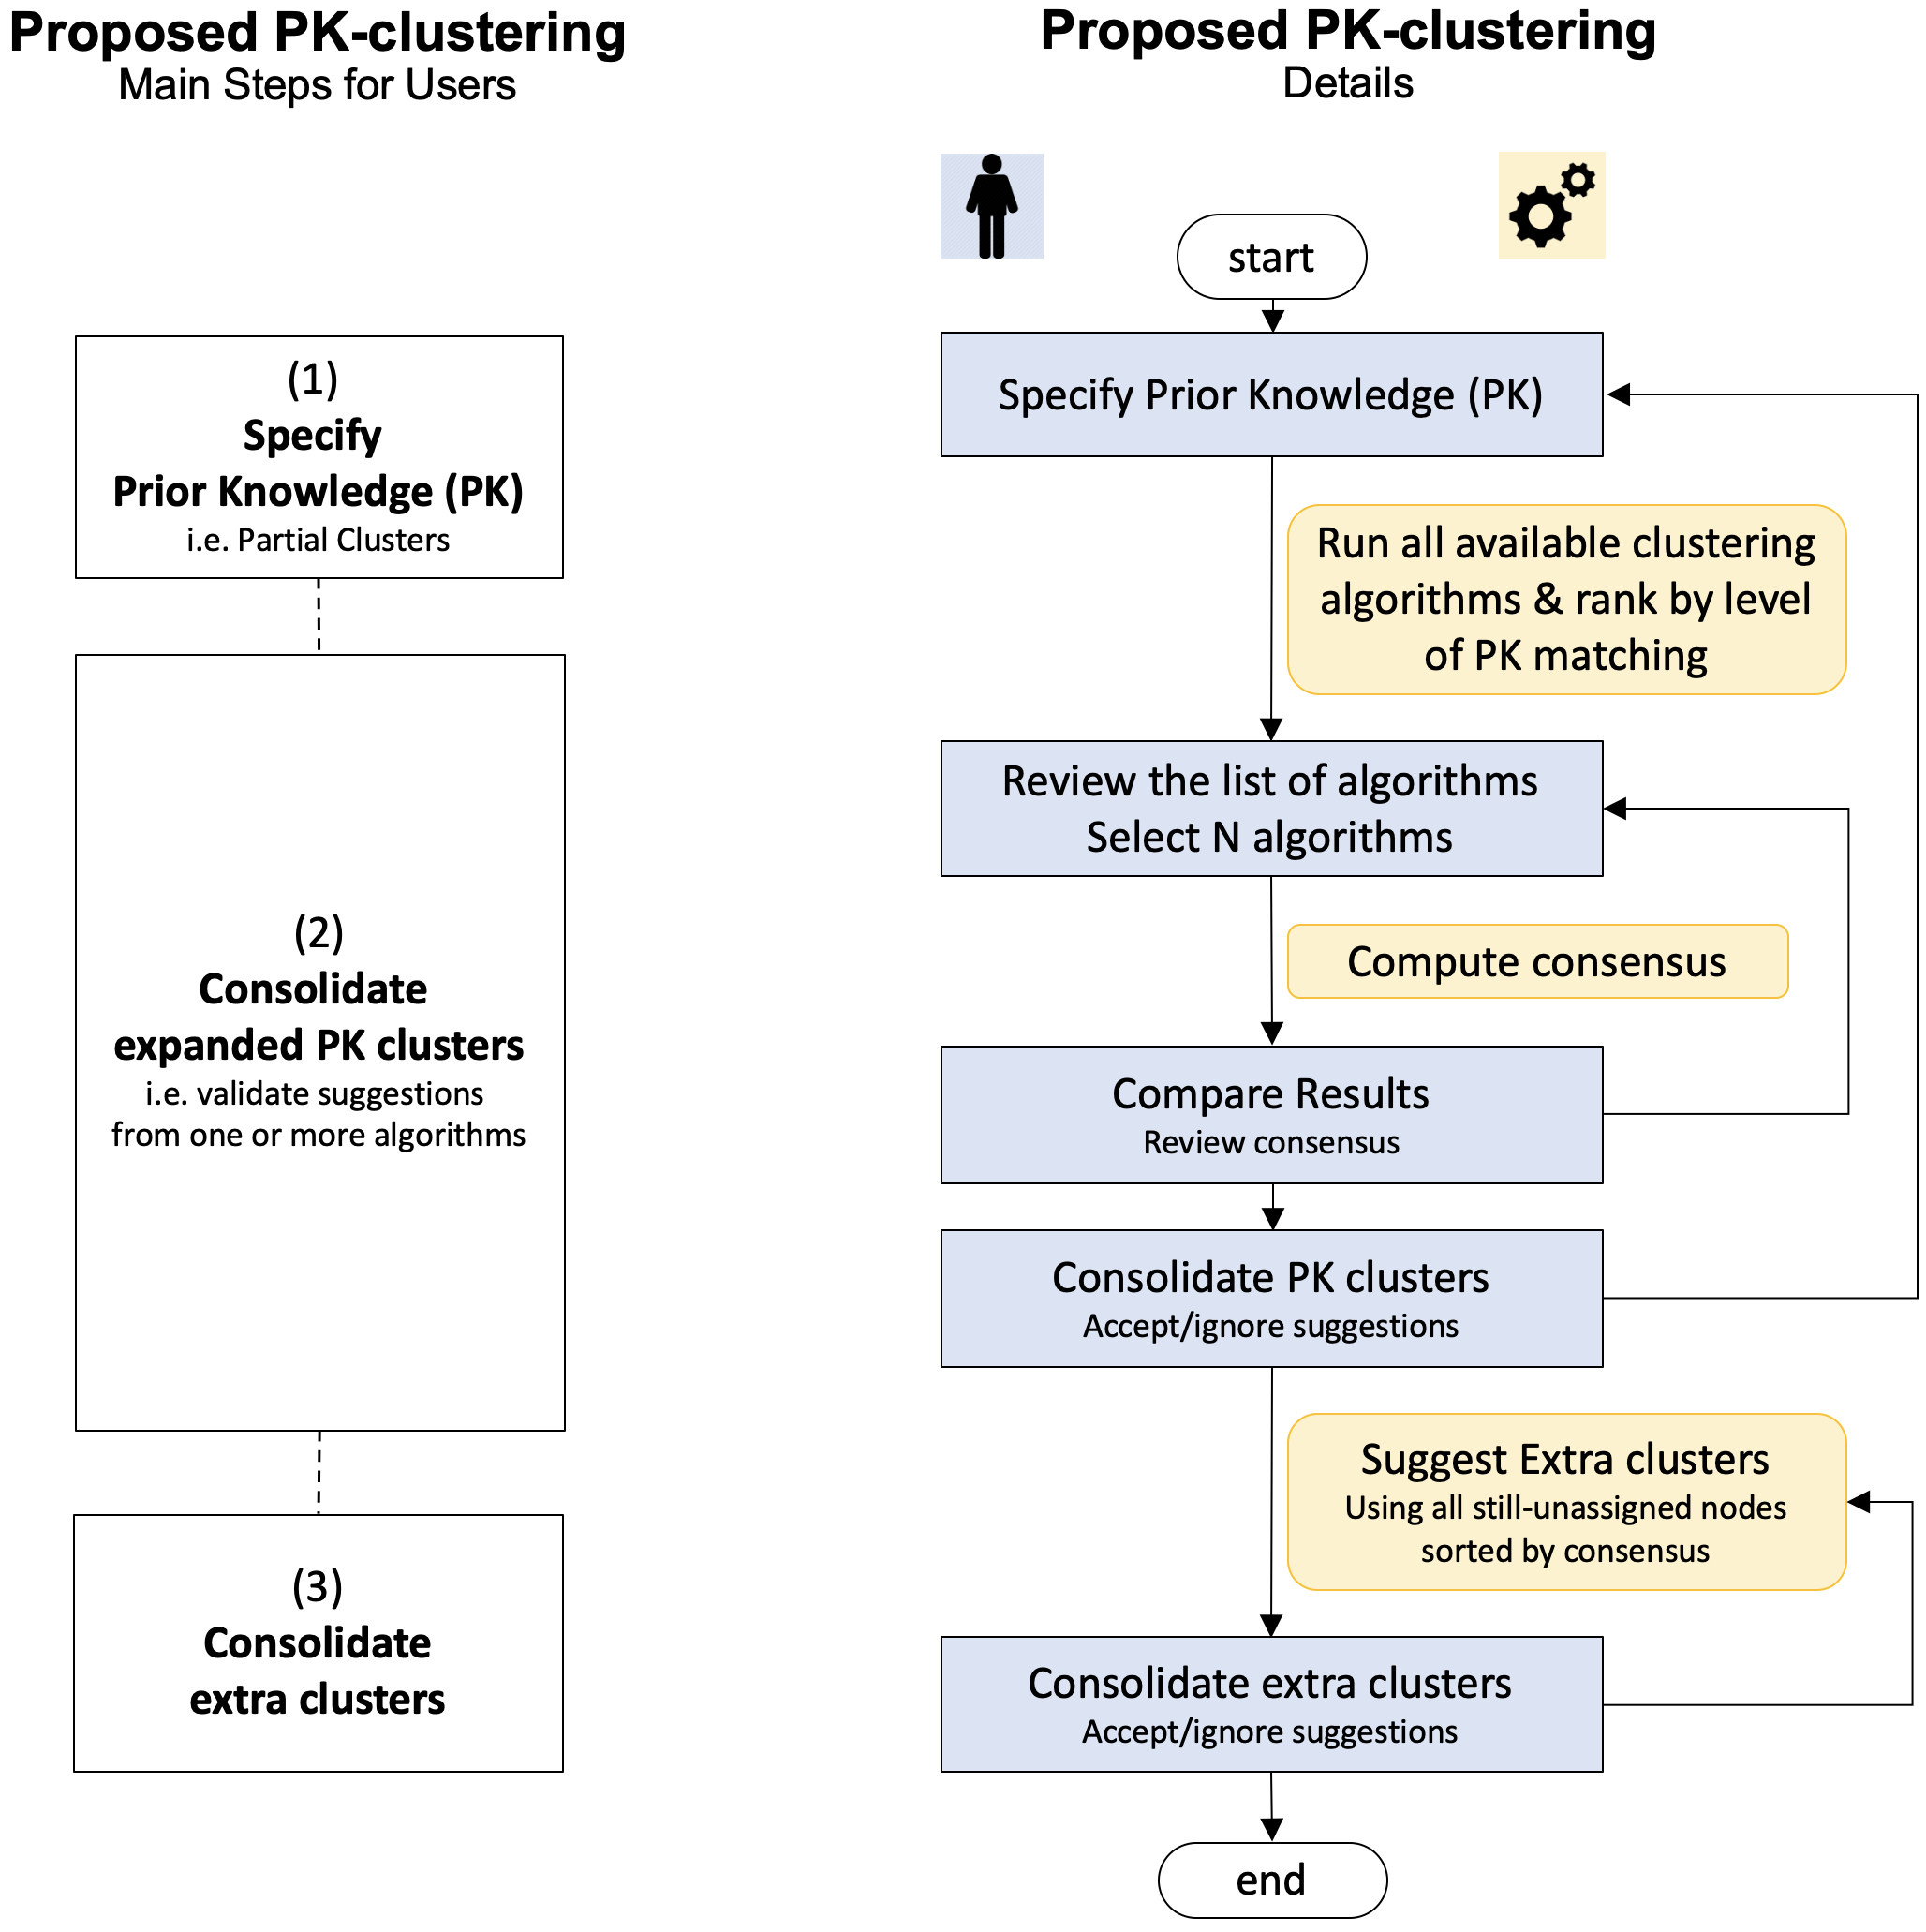
\includegraphics[width=\columnwidth]{static/figures/PK-Clustering/VISPaperFigures/pkprocess_new.png}
    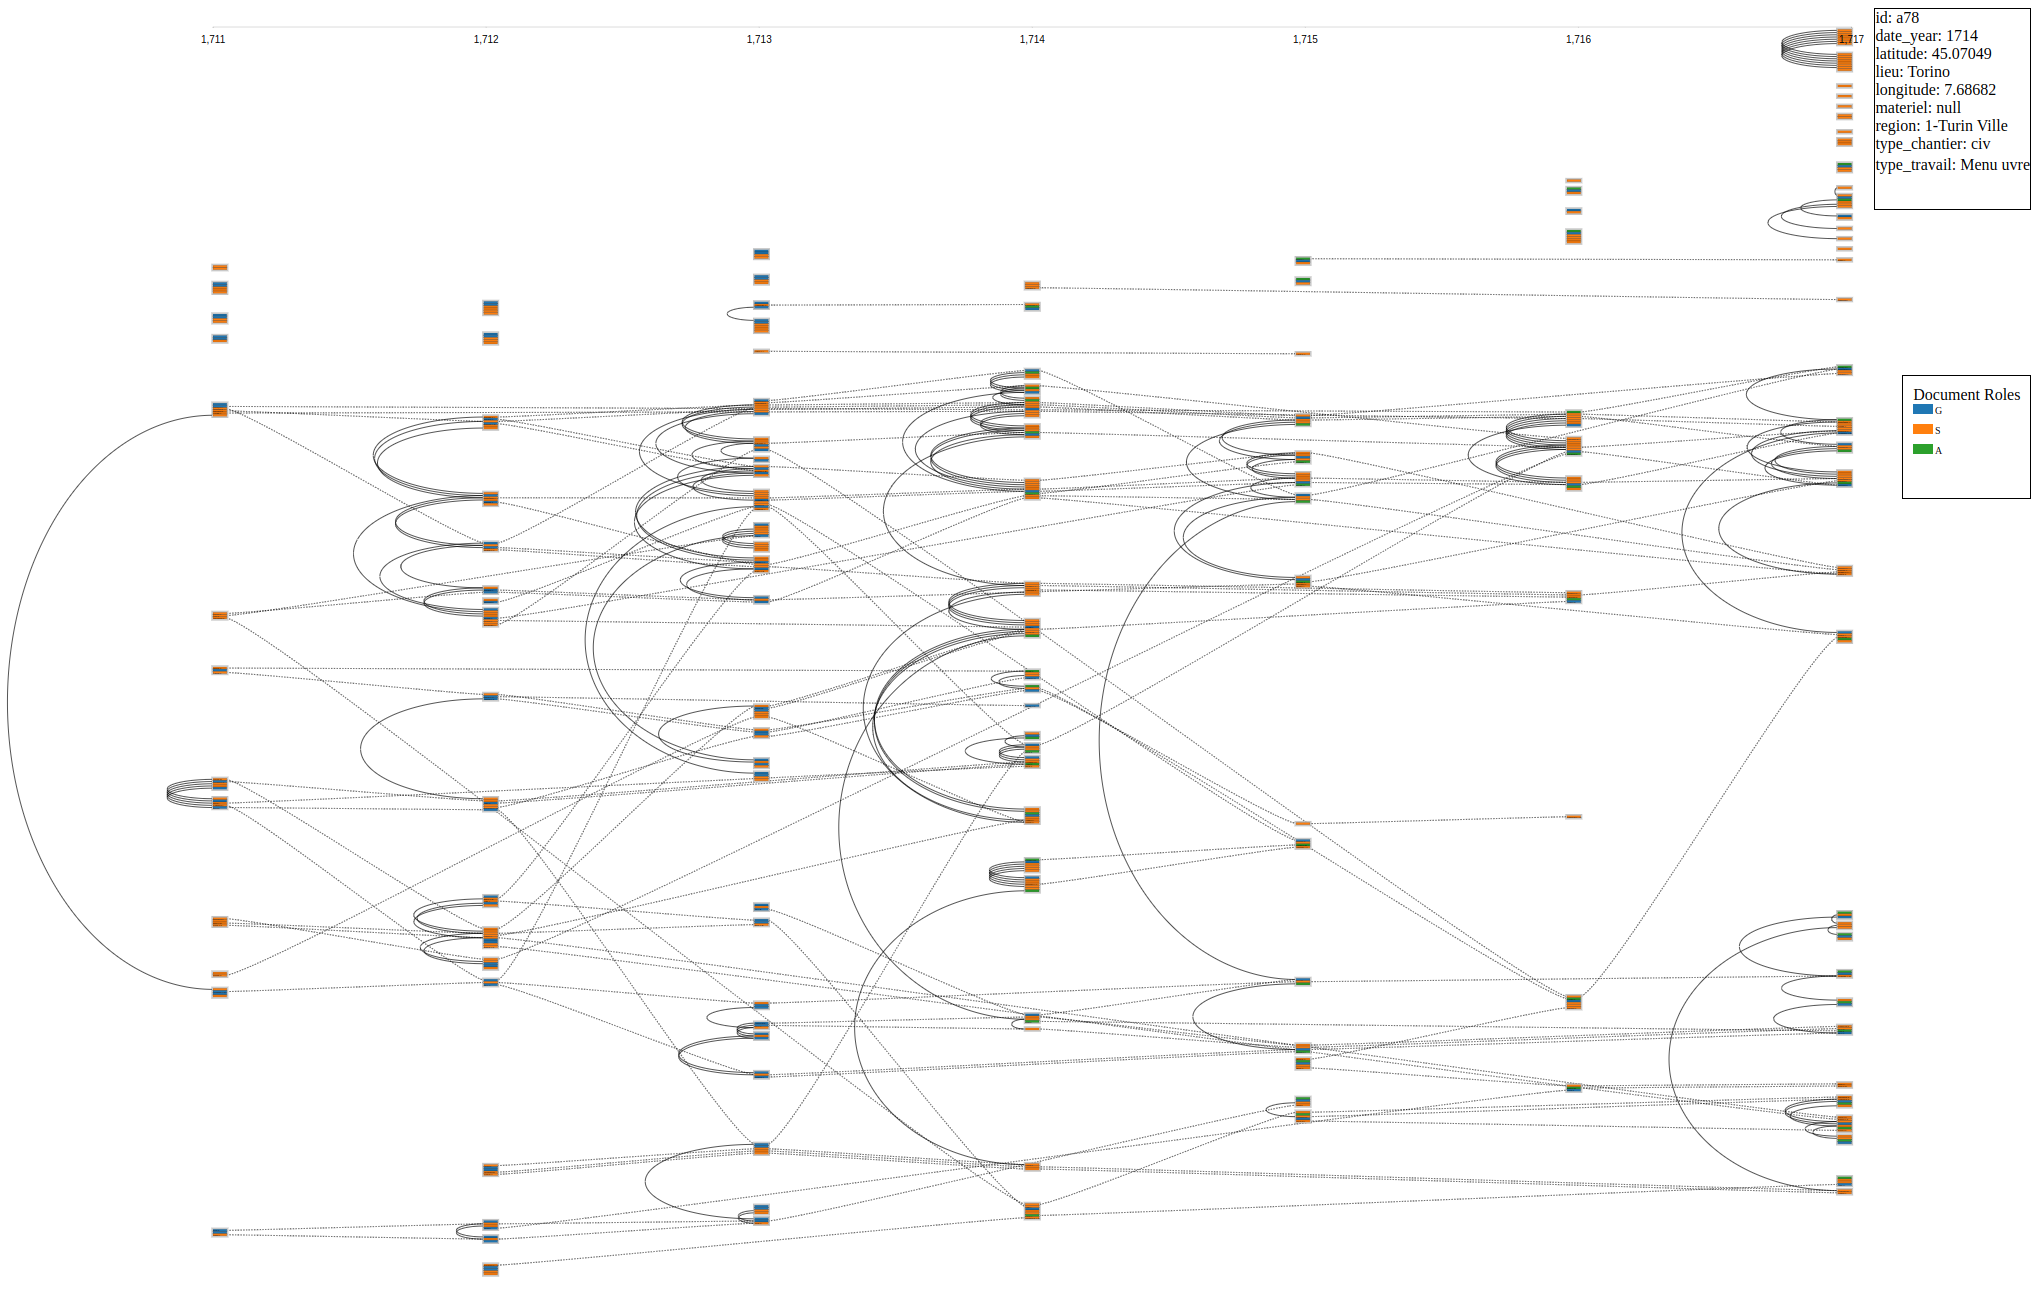
\includegraphics[width=\textwidth]{static/figures/conclusion/dyn2}
    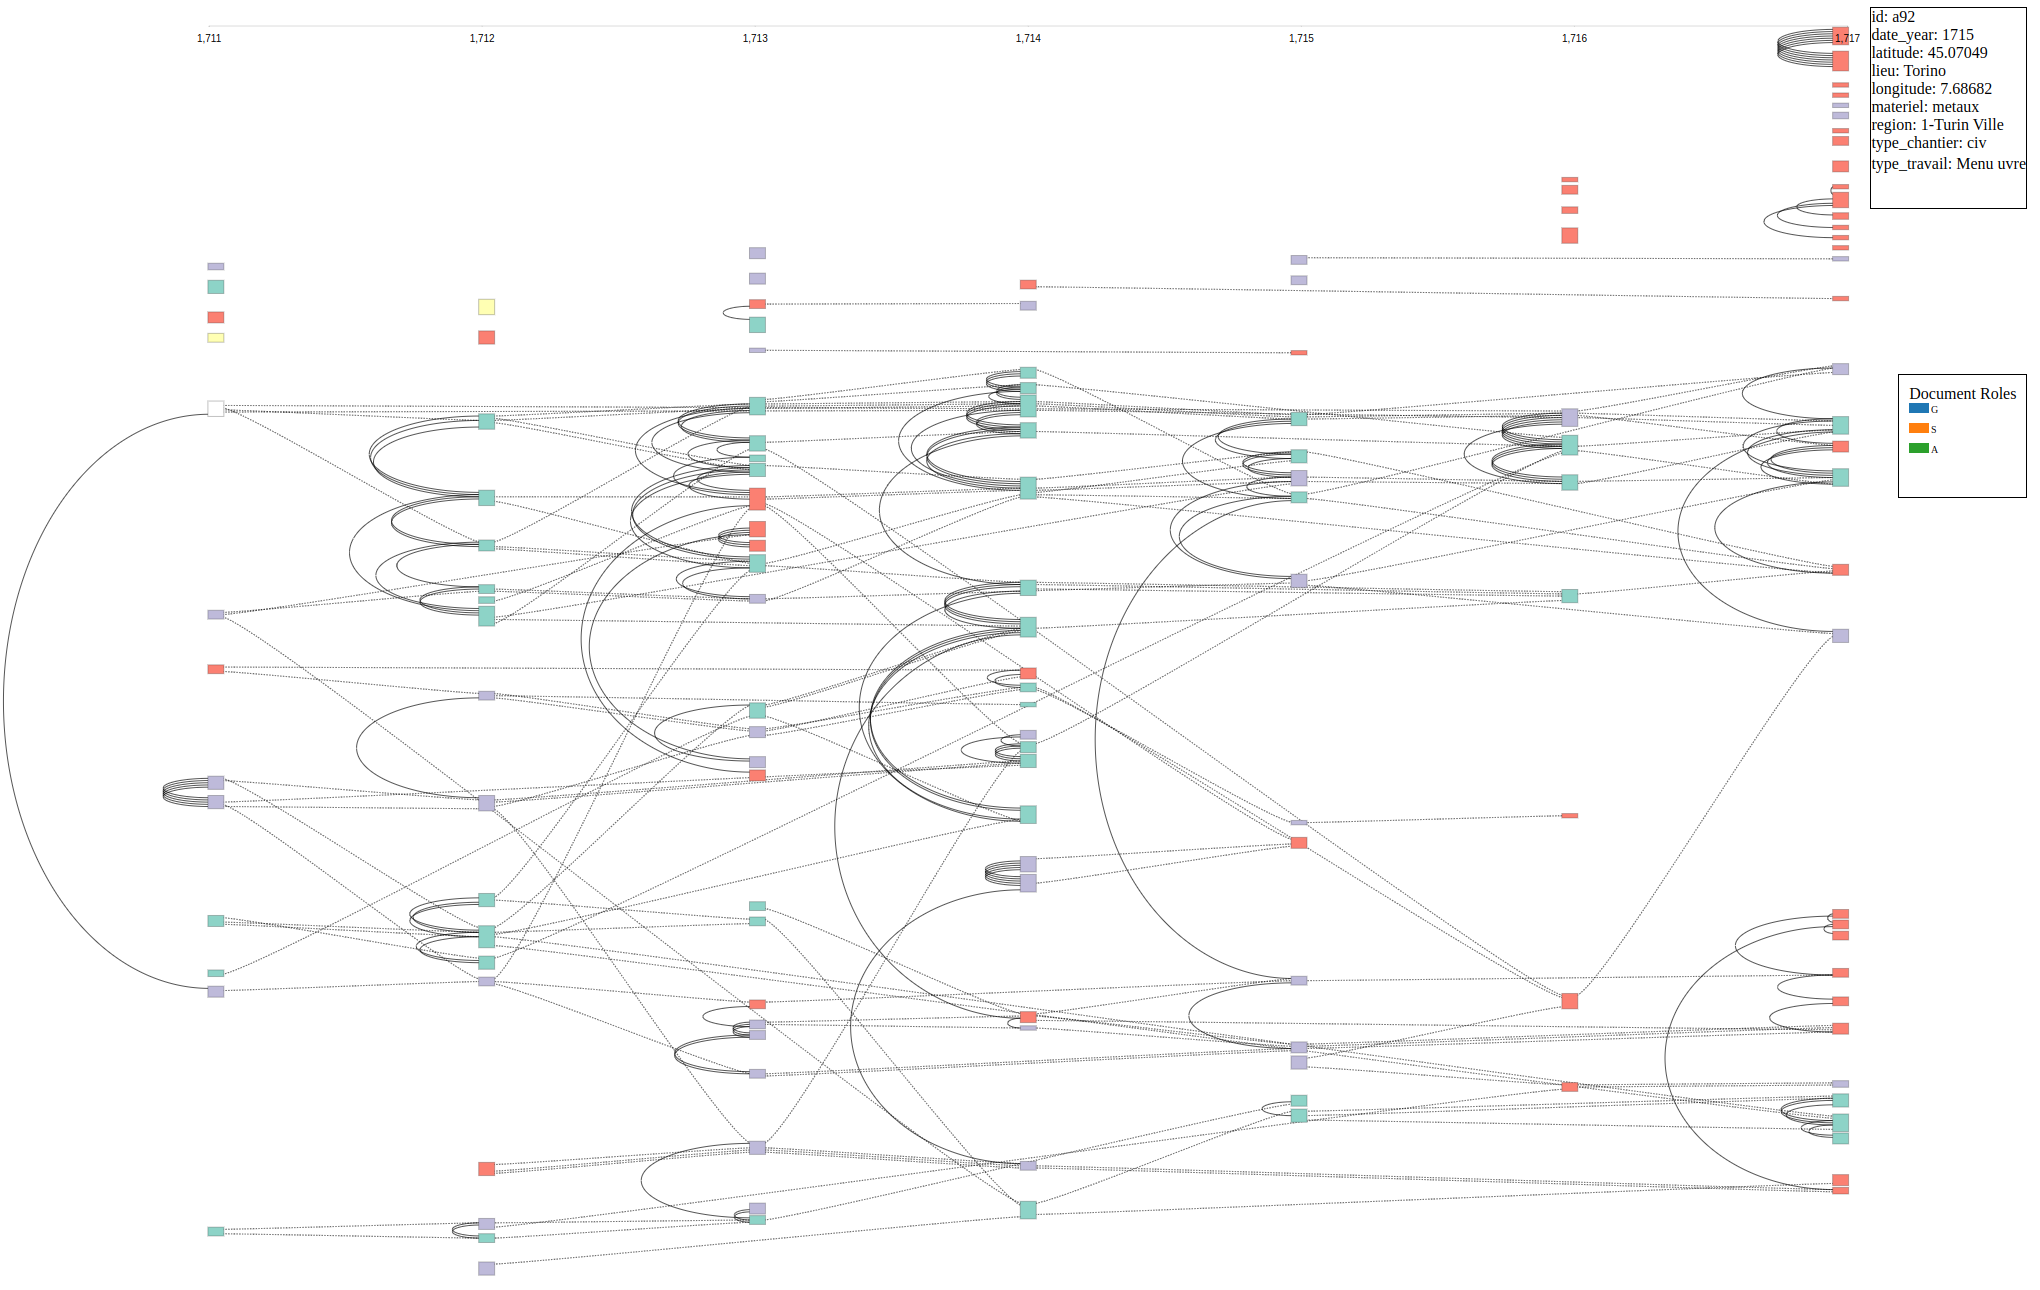
\includegraphics[width=\textwidth]{static/figures/conclusion/dyn2_region}
    \caption{Prototype of a document-centered dynamic layout for \modelplural, visualized with data of construction contracts in Piedmont (see collaboration \pascal in \autoref{ch:hsna-process-and-network-modeling}). The layout can show the mention of persons encoded with their roles (top) or the documents and their properties (bottom). Here, the \emph{region} attribute is selected, hence coloring construction contract depending on their location.}
\label{fig:conclu-dynLayout}
\end{figure}

This layout prototype could serve as a base to develop a process similar to \pkclustering, but for creating meaningful dynamic groups, based on the consensus of dynamic clustering algorithms, prior knowledge of social historians, and exploration capabilities.
%As with static clustering, the results produced by algorithms can be biased, and several interesting dynamic partitions coexist.
%A similar procedure of PK-Clustering but with dynamic clustering would mitigate those problems, by providing a way to construct meaningful clusters for social scientists using their prior-knowledge, algorithmic consensus, and exploration capabilities.



\noindent\textbf{Machine Learning, automation, and agency.} Machine learning went through rapid progress in the last 10 years, mainly due to the increase of data storage, computing power, and the rise of deep learning architectures.
It has been applied to various tasks such as automatic driving, fraud detection, computer vision, and medical diagnostics.
In the context of \sna, machine learning methods have been used to automatically extract knowledge through tasks such as node classification, clustering, and link prediction\cite{michalskiPredictingSocialNetwork2012}.
More broadly, it has also been used for historical document digitization\cite{philipsHistoricalDocumentProcessing2020}.
If machine learning can give state-of-the-art accuracy on many of those tasks, it also poses issues with the explainability and reliability of the results in real-world applications.
It can be particularly frustrating in the context of social history, as historians need to be able to understand and explain the structure of their networks, as discussed in \autoref{ch:pk-clustering}.
Several methods and approaches now focus on trying to explain the outputs of these black-box algorithms to the end user\cite{holzingerMachineLearningExplainable2018}.
Similarly, research is done on how to design interactive systems which leverage machine learning algorithms to guide and advise users, which are at the center of the decision-making process.
This concept of utilizing artificial intelligence power to support human decision-making through interactive systems has been coined as ``agency''\cite{heerAgencyAutomationDesigning2019} and ``human-centered artificial intelligence''\cite{shneidermanHumanCenteredAI2022}.
PK-clustering is based on the core idea that machine learning should support users while not removing their decision-making process, by providing automatic suggestions through clustering results, while letting social historians decide.
\name could also be extended with machine learning agency, for example, to suggest social scientists recurring subgraphs in the data, that could be interesting to them.
Over-represented subgraphs could be a query start that the users would refine through the easy-to-use visual query system.
This idea of human-centered artificial intelligence could be applied not only to the analysis part but also to the data preparation workflow, for example in document transcription, named entity recognition, and disambiguation, all tasks that machine learning is efficient at.

%A lot of work has been done in the recent years on machine learning, due to its rapid progress in various tasks such as questions answering, automatic driving, fraud detection, or node classification.
%Machine learning has also been applied to social sciences and DH, for example for historical documents digitization \cite{philipsHistoricalDocumentProcessing2020}, or link prediction \cite{michalskiPredictingSocialNetwork2012}.
%Machine learning can give state-of-the-art accuracy on many of those tasks, but often set issues on the explainability and reliability of the results in real world applications.
%Several methods and approaches now focus on trying to explain the results of those black-box algorithms to the end-user.
%Similarly, research is done on how to design interactive systems which leverage machine learning algorithms to guide and advise users, who still have to take the main decisions \cite{heerAgencyAutomationDesigning2019}.
%PK-clusterering is based on this idea that machine learning should help users make decision based on automatic computations while letting them at the center of the analysis loop.
%\name could also be extended with machine learning features and with the same agency idea, for example to suggest social scientists recurring subgraphs in the data, that could be interesting to them.
%The over represented subgraphs could be a query start that the users could refine.
%
%This idea of empowering users with the help of machine learning algorithms could be extended to the overall workflow of social historians.
%In their workflow, as we saw in \autoref{ch:hsna-process-and-network-modeling} they have to manually do various tasks like transcription, Named Entity Recognition, and Named Entity Disambiguation that machine learning is efficient at.
%VA interfaces could help social scientists do these tasks more easily by providing help and suggestions from  machine learning results and interactions.


\noindent\textbf{A common workflow interface.} Currently, most social scientists have to use a lot of different pieces of software, files, and ad-hoc processes to follow quantitative analyses.
I provided two \va interfaces to help historians analyze their data and ease back and forth between the different steps of their analysis.
Both interfaces use the same data format to lower the time cost to switch between them.
However, historians still have to collect and annotate/encode their data manually with ad-hoc methods and may have to convert their data to various formats when using several visual analysis tools.
All these operations usually break the traceability and reproducibility of their analyses, and make their process tedious, especially since it often requires the writing of conversion scripts, which they do not necessarily have the programming skills to do.
I, therefore, argue there is a need for visual interfaces which integrate the whole workflow of social scientists, from the data collection to the formulation of high-level conclusions.
If all the processes they do is integrated into the same visual environment, it would ease the flow of the analysis, increase the traceability and replicability of the actions and results, and allow them to take several exploration paths more easily.
\combinet and \pkclustering could for example be integrated into the same environment, with added possibilities of managing documents in the same place, applying annotations/encoding, and seeing in real-time the creation of networks and transformations from the annotation process instead of having to do many back and forth.
This constitutes an interesting research direction as it would allow social historians to collect, annotate, apply transform, analyze, and visualize their historical documents in the same environment, with easy-to-use interactions and artificial intelligence support.


%In the contrary, if all the processes they do is integrated in the same visual environment, it would ease the flow of the analysis, increase the traceability of the results and actions, and allow them to take several explorations paths more easily.
%An interesting research direction would be to develop such systems, allowing social historians to collect, annotate, apply transform, analyse, and visualize their historical documents in the same environment, with easy-to-use interactions and artificial intelligence support.
%This would tremendously ease back and forth between the different \hsna steps, thus allowing better exploration of different analysis paths, while enhancing the traceability/replicability of results and the grounding of high-level conclusions back to the original historical sources.



\section{Conclusion}


To conclude, the goal of this thesis was to provide answers and directions towards the question of how \va, and more globally computer science, can help and support historians in the analyses they want to make.
Towards this goal, I first formalized the current \hsna process from collaborations and discussions, defined three properties tools supporting this process should satisfy (\emph{traceability}, \emph{simplicity}, and \emph{document reality)}, and proposed two interfaces showcasing visualization and interactions mechanisms to support social historian in their workflow, leveraging historical documents modeled as \modelplural.
\combinet allows users to explore this data model, reflect on annotations, reveal specific facets of the data, and globally highlight and compare specific groups and behaviors to either detect erroneous patterns or answer socio-historical questions.
\pkclustering aims at integrating better the clustering task in the social historians' workflow, by providing a mixed-initiative approach for clustering on \modelplural leveraging the prior knowledge of practitioners, the consensus of automatic algorithms, and exploration capabilities.
Both systems have been validated with real use cases, and aim at providing simple-to-use yet expressive tools, which let historians at the center of the analysis loop.
Indeed, the use of quantitative methods in history and more globally the humanities has led to many expectations in the last 50 years, but also many disappointments due to usability and interpretability issues.
More recently, with the rise of popularity of machine learning, many propositions are made towards automatic inspection and extraction of historical data.
Yet, much criticism emerged towards those methods, as they can easily lead to disembodied work without a deep understanding of historical content and phenomena.
Moreover, historians actually regard highly the inspection process of the sources.
As one historian told me, ``What many people promoting artificial intelligence to automatically read and inspect historical sources do not understand, is that this part is actually the most fun aspect of the historical work, and why many of us do it.''
Computer-supported tools for digital humanities should therefore support practitioners with the help of interactive visualization and quantitative-supported suggestions, instead of only providing automatic uninterpretable results.
Propositions of this work aim in this direction, which I think is where lies the future of digital humanities as a field, \ie methods, and systems that social scientists can use easily with low friction and entry barriers, which provide data-supported suggestions to help the decision-making process of scientists through visualization and interaction.





